% Centri — Weekly progress (week ending 2026-07-08)
% New evaluation method, adapted from Utami (2025). Compile: pdflatex -interaction=nonstopmode ... (run twice)
\documentclass[aspectratio=169,10pt]{beamer}
\usetheme{metropolis}
\metroset{sectionpage=progressbar, subsectionpage=none, numbering=fraction, progressbar=frametitle}

\usepackage{booktabs}
\usepackage{amsmath,amssymb}
\usepackage{siunitx}
\usepackage{xcolor}
\usepackage{colortbl}
\usepackage{graphicx}
\graphicspath{{figs/}}
\usepackage{tikz}
\usetikzlibrary{arrows.meta,positioning,calc,shapes.geometric,fit,backgrounds}
\usepackage[most]{tcolorbox}

% ---- palette (shared with the other Centri decks) ------------------------
\definecolor{cMeas}{HTML}{1F6FB2}
\definecolor{cPed}{HTML}{B5651D}
\definecolor{cApp}{HTML}{2E7D32}
\definecolor{cInfra}{HTML}{5E35B1}
\definecolor{cAccent}{HTML}{C62828}
\definecolor{cGrey}{HTML}{616161}
\definecolor{cBg}{HTML}{F4F6F8}
\definecolor{cBasic}{HTML}{2E7D32}
\definecolor{cInter}{HTML}{1565C0}
\definecolor{cAdv}{HTML}{6A1B9A}
\setbeamercolor{frametitle}{bg=cMeas}
\setbeamercolor{progress bar}{fg=cAccent}

\newcommand{\hl}[1]{{\bfseries\color{cAccent}#1}}
\newcommand{\ok}{{\color{cApp}\textbf{\checkmark}}}

\tikzset{
  box/.style={rounded corners=2pt, draw=#1, line width=0.8pt, fill=#1!8,
              text=black, align=center, font=\scriptsize, inner sep=4pt, minimum height=8mm},
  node distance=5mm and 8mm,
  flow/.style={-{Stealth[length=2.2mm]}, line width=0.7pt, draw=cGrey},
}

\title{Centri --- A New Evaluation Method}
\subtitle{Adapting the parent line's (2025) multi-axis evaluation to tiered physics material}
\author{Damar Albaribin}
\institute{MSc Thesis --- advisor: Prof.\ Wu-Yuin Hwang}
\date{Week ending 2026-07-08}

\begin{document}
\maketitle

% =========================================================================
\begin{frame}{Where this comes from --- and what's in place}
\small
\begin{tcolorbox}[colback=cGrey!8,colframe=cGrey,title=\footnotesize The gap this fills,boxsep=2pt,left=4pt,right=4pt]
\scriptsize
A similarity metric alone misses the quality axes: \emph{``LLM-judge $+$ teacher panel
(lab rubric: linguistic $+$ mathematical), $\kappa$ vs.\ humans, auto$\leftrightarrow$human Pearson.''}
Those come from the \textbf{parent line} --- \textbf{Ika Q.\ Utami's PhD} (NCU, same advisor):
\emph{Authentic MWP Generation with Generative AI}. Its \textbf{SocioMathLLM} study defines the
LLM-judge $+$ rubric (Tables 8--10) and \textbf{Geo-QG} the 3-tier design --- exactly what Centri
should inherit so our numbers sit \textbf{beside the lab's published ones}.
\end{tcolorbox}
\vspace{0.2em}
That gap is now a real, wired evaluation method:
\begin{itemize}\setlength\itemsep{1pt}
  \item \textbf{\color{cMeas}Rubric adopted verbatim} \ok\ --- SocioMathLLM's Tables 8--9 (authenticity/linguistic
  $+$ mathematical) drive our LLM-judge and a teacher rating sheet, plus a Centri physics/tier block.
  \item \textbf{\color{cPed}The parent line's correlation layer} \ok\ --- Cohen's $\kappa$, ICC, Pearson
  in one tool (\texttt{eval\_stats.py}).
  \item \textbf{\color{cApp}Preliminary numbers in hand} \ok\ --- 15 passages judged on the new rubric;
  the tier ladder shows up in the scores. The teacher panel is the one axis not yet run.
\end{itemize}
{\footnotesize The code $+$ docs are in place; the full production run and teacher panel are the remaining steps.}
\end{frame}

% =========================================================================
\section{Why a new evaluation method}

\begin{frame}{BERTScore/BLEU measure overlap, not pedagogy}
\small
Our headline metric so far is \textbf{BERTScore vs a reference}, and its blind spot is
concrete: on all 5 objects, \hl{basic scores \emph{lowest}} --- not because it is worse, but
because it has the fewest equation-like tokens to overlap with an equation-dense textbook.
\vspace{0.4em}
\begin{tcolorbox}[colback=cAccent!6,colframe=cAccent,boxsep=2pt,left=5pt,right=5pt]
\small BERTScore/BLEU measure \textbf{lexical / element density}, not whether a passage is a
\emph{good lesson}. A pedagogy-aware evaluation needs axes they do not have.
\end{tcolorbox}
\vspace{0.5em}
The parent dissertation solves precisely this with a \textbf{multi-axis} method (§2.4, §3.4.3):
automatic metrics for comparability, an \textbf{expert-teacher rubric} for pedagogy, an
\textbf{LLM-as-judge} on the same rubric, and \textbf{correlation statistics} tying them together.
We adopt it wholesale and optimise for our case (tiers $+$ physics $+$ our grounding gate).
\end{frame}

\begin{frame}{The method: four axes, then correlate}
\scriptsize
\begin{center}
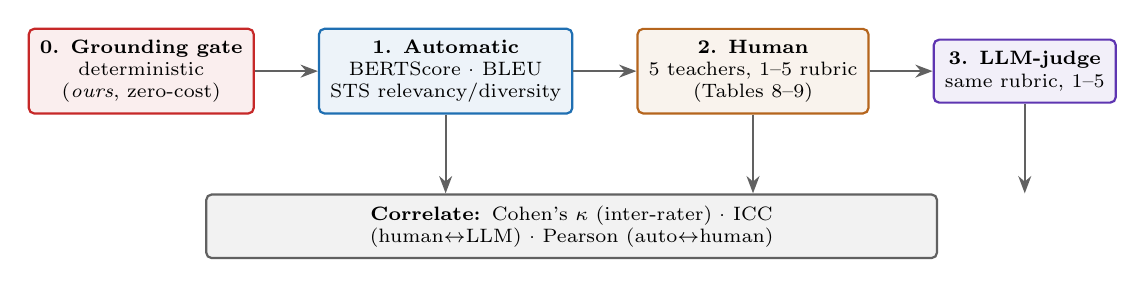
\begin{tikzpicture}
\node[box=cAccent] (gate) {\textbf{0. Grounding gate}\\deterministic\\(\emph{ours}, zero-cost)};
\node[box=cMeas, right=of gate] (auto) {\textbf{1. Automatic}\\BERTScore · BLEU\\STS relevancy/diversity};
\node[box=cPed, right=of auto] (human) {\textbf{2. Human}\\5 teachers, 1--5 rubric\\(Tables 8--9)};
\node[box=cInfra, right=of human] (llm) {\textbf{3. LLM-judge}\\same rubric, 1--5};
\draw[flow] (gate)--(auto); \draw[flow] (auto)--(human); \draw[flow] (human)--(llm);
\node[box=cGrey, text width=9cm, below=10mm of auto, xshift=1.6cm] (stat)
  {\textbf{Correlate:} Cohen's $\kappa$ (inter-rater) · ICC (human$\leftrightarrow$LLM) ·
   Pearson (auto$\leftrightarrow$human)};
\draw[flow] (auto.south) -- (auto.south|-stat.north);
\draw[flow] (human.south) -- (human.south|-stat.north);
\draw[flow] (llm.south) -- (llm.south|-stat.north);
\end{tikzpicture}
\end{center}
\vspace{0.3em}
\begin{itemize}\setlength\itemsep{2pt}
  \item Axes \textbf{1--3} are the parent line's, kept verbatim for comparability. Axis \textbf{0} is
  Centri's extra intrinsic layer --- the deterministic grounding gate runs first, for free, and no prior
  work in the SLR has it.
  \item \textbf{Our optimisation:} tier-matched references (not one fixed reference), and per-tier
  \textbf{difficulty-fit $+$ achieved-Bloom} fed the gate's own EI/Bloom labels as ground truth.
  \item \textbf{Headline vs comparability:} LLM-judge $+$ teacher rubric are the headline (pedagogy);
  BERTScore/BLEU are the comparability baseline --- as argued in Study 4 (SocioMathLLM).
\end{itemize}
\end{frame}

% =========================================================================
\section{The rubric we adopted}

\begin{frame}{SocioMathLLM's Tables 8--9, verbatim --- plus a Centri tier block}
\scriptsize
Every dimension scored \textbf{1--5}. Source of truth: \texttt{docs/eval-rubric-ika.md}
--- shared by the LLM-judge \emph{and} the teacher sheet, so both score the same criteria.
\vspace{0.3em}
\renewcommand{\arraystretch}{1.35}
\begin{center}
\begin{tabular}{@{}p{2.7cm}p{2.0cm}p{7.2cm}@{}}
\toprule
\textbf{Axis} & \textbf{Source} & \textbf{Dimensions (each 1--5)} \\
\midrule
\textbf{\color{cPed}Authenticity / linguistic} & SocioMathLLM Table 8 &
motivating context · language \& cultural clarity · appropriate \# solution steps ·
variety of solution strategies · cognitive demand \\
\textbf{\color{cMeas}Mathematical} & SocioMathLLM Table 9 &
problem answerability · structure \& clarity · multiple solution strategies \\
\textbf{\color{cApp}Physics / tier} & Centri \emph{(ours)} &
difficulty\_fit (basic/int/adv) · concept\_accuracy · grounding\_accuracy ·
achieved\_bloom (vs the tier's designed Bloom) \\
\bottomrule
\end{tabular}
\end{center}
\vspace{0.5em}
\begin{itemize}\setlength\itemsep{2pt}
  \item Table 10 (\textbf{socialization}) is \emph{intentionally not} adopted --- it is the SocioMathLLM
  (Study 4) contribution, outside Centri's lane.
  \item BLEU is read on the parent line's interpretation scale (§3.2.4): $<$1 undesired $\ldots$ 4--5 high
  quality $\ldots$ $>$6 better-than-human.
\end{itemize}
\end{frame}

\begin{frame}{The evaluation tooling in place}
\small
\renewcommand{\arraystretch}{1.25}
\begin{center}
\begin{tabular}{@{}p{3.5cm}p{7.5cm}@{}}
\toprule
\textbf{Tool} & \textbf{What it does} \\
\midrule
\texttt{run\_llm\_judge.py} & LLM-judge re-aligned to SocioMathLLM Tables 8--9 $+$ tier block; can take the
gate's measured EI as ground truth. \\
\texttt{eval\_stats.py} & Cohen's $\kappa$ $+$ \% agreement, ICC(2,k), Pearson --- the parent line's
§3.4.3 correlation layer, numpy-only, tidy-CSV in. \\
\texttt{build\_rater\_sheet.py} & Emits one CSV per teacher (item $\times$ rubric row),
ingestible \emph{unchanged} by \texttt{eval\_stats.py}. \\
\texttt{generate\_tier\_material.py} & \hl{\texttt{-{}-candidates K}}: generate-K, gate-select the
cleanest draft (SocioMathLLM's generate$\to$review$\to$select) --- the durable fix for the 35B
self-correction limit. \\
\midrule
\multicolumn{2}{@{}l}{\scriptsize\textbf{Docs:} \texttt{eval-rubric-ika.md},
\texttt{related-work-positioning.md}, \texttt{effectiveness-study-blueprint.md}} \\
\bottomrule
\end{tabular}
\end{center}
\vspace{0.3em}
{\footnotesize Default behaviour unchanged (\texttt{-{}-candidates 1}); the human pipeline is wired,
pending teacher scores.}
\end{frame}

% =========================================================================
\section{Preliminary results}

\begin{frame}{The rubric already sees the tier ladder (preliminary)}
\scriptsize
\textbf{5 objects $\times$ 3 tiers $=$ 15 passages}, from existing outputs, judged by the lab Qwen
on the new rubric. \emph{Preliminary/illustrative --- no teacher ratings yet.}
\vspace{0.2em}
\renewcommand{\arraystretch}{1.2}
\begin{columns}[T]
\begin{column}{0.5\textwidth}
\centering{\scriptsize\bfseries LLM-judge axis means (1--5)}\\[2pt]
\begin{tabular}{@{}lccc@{}}
\toprule
\textbf{Axis} & \color{cBasic}basic & \color{cInter}interm. & \color{cAdv}adv. \\
\midrule
authenticity/ling. & 2.56 & 2.92 & \textbf{3.40} \\
mathematical & 2.13 & \textbf{3.33} & 2.67 \\
physics/tier & \textbf{4.07} & 3.80 & 2.47 \\
\bottomrule
\end{tabular}
\end{column}
\begin{column}{0.5\textwidth}
\centering{\scriptsize\bfseries Criteria that \emph{should} rise with tier}\\[2pt]
\begin{tabular}{@{}lccc@{}}
\toprule
\textbf{Criterion} & \color{cBasic}basic & \color{cInter}int. & \color{cAdv}adv. \\
\midrule
cognitive\_demand & 2.2 & 2.6 & \textbf{4.0} \\
solution\_steps & 1.2 & 2.0 & \textbf{3.0} \\
achieved Bloom & \multicolumn{2}{c}{Understand} & \textbf{Analyze} \\
\bottomrule
\end{tabular}
\end{column}
\end{columns}
\vspace{0.5em}
\begin{tcolorbox}[colback=cApp!6,colframe=cApp,boxsep=2pt,left=5pt,right=5pt]
\scriptsize \textbf{\color{cApp}The ladder is visible in an independent model's scores}: cognitive
demand $2.2\to4.0$, solution steps $1.2\to3.0$, achieved Bloom Understand $\to$ Analyze at advanced
(4/5 cases). This is the pedagogy signal BERTScore could not give.
\end{tcolorbox}
\end{frame}

\begin{frame}{Honest reading of the preliminary numbers}
\small
Three findings worth flagging (they shape the full production run):
\begin{itemize}\setlength\itemsep{4pt}
  \item \hl{Grounding drops at advanced} (grounding\_accuracy $4.4\to3.6\to1.0$). The advanced
  tier makes per-instant numeric claims; on oblique-capture clips those cannot be verified ---
  the \emph{same} limitation the deterministic gate flags. A real result, not noise.
  \item \textbf{The mathematical axis is expository-unfair.} Dimensions like ``\# solution steps''
  and ``multiple strategies'' assume a \emph{problem to solve}; our material is \emph{exposition}.
  Basic scores low there by construction --- reported honestly, and noted as the one place the
  question-rubric doesn't map cleanly onto passages.
  \item \textbf{EI monotonicity fails 4/5} (intermediate overshoots advanced) --- advanced trades
  \emph{breadth} of quantities for \emph{depth}. FK grade rises for all 5.
\end{itemize}
\vspace{0.3em}
\begin{tcolorbox}[colback=cMeas!6,colframe=cMeas,boxsep=2pt,left=4pt,right=4pt]
\scriptsize Automatic (comparability) baseline held: BERTScore \textbf{F1 $=0.830\pm0.014$} (n$=$75),
whole-passage F1 $=0.823$, diversity $0.311$.
\end{tcolorbox}
\end{frame}

% =========================================================================
\begin{frame}{Where the method stands}
\small
\begin{columns}[T]
\begin{column}{0.52\textwidth}
\textbf{\color{cApp}In place}
\begin{itemize}\setlength\itemsep{1pt}\small
  \item Rubric adopted from SocioMathLLM Tables 8--9 \ok
  \item LLM-judge re-aligned to it $+$ tier block \ok
  \item \texttt{eval\_stats.py}: $\kappa$ / ICC / Pearson \ok
  \item Teacher rating-sheet generator \ok
  \item Generate-K-gate-select loop (35B fix) \ok
  \item SLR positioning $+$ effectiveness-study docs \ok
  \item Preliminary judge run, 15 passages \ok
\end{itemize}
\end{column}
\begin{column}{0.48\textwidth}
\textbf{\color{cAccent}Open --- not yet run}
\begin{itemize}\setlength\itemsep{1pt}\small
  \item \textbf{Teacher rating sheets deployed} $\rightarrow$ real Cohen's $\kappa$, ICC
        (human$\leftrightarrow$LLM), Pearson (auto$\leftrightarrow$human)
  \item Full production run with \textbf{tier-matched references}
  \item \textbf{Candidate-select K} tuned (does best-of-K reach 15/15 clean?)
  \item Effectiveness study, per the Study-3 blueprint (needs IRB $+$ app instrumentation)
\end{itemize}
\end{column}
\end{columns}
\vspace{0.6em}
\begin{center}
{\footnotesize\itshape The parent line's evaluation method is inherited, wired end-to-end, and
already sees the difficulty ladder --- the teacher panel is what turns preliminary into publishable.}
\end{center}
\end{frame}

\end{document}
